%!TEX root = ../../../super_main.tex

\chapter{Issues and Solutions}
\label{sec:sprintone_issues_solutions}
The \launcher application seems to be working fine at a first glance, but at further inspection reveals that it has a lot of edge cases that cause it to crash when used for longer periods of time. In order to find these crashes we conducted a series of unstructured tests and UI/Application Exerciser Monkey (Monkey) \parencite{android_monkey} tests to explore the \launcher and find bugs during the start of the first sprint. Monkey is a tool, which comes with the Android Debug Bridge (adb) \parencite{android_adb}, used to perform series of pseudo-random streams of user events to test the application UI under stress. We found the Monkey tool to be useful and it did help us find several issues in the code, e.g. concurrency issues when switching between tabs in the settings activity of the \launcher.
\\\\
Android and general code mistakes might occur multiple times in codebase, and will be corrected when discovered, but only the first discovered occurrence is mentioned in this chapter. 
\\\\
In addition to the issues discovered by using the Monkey tool, some requests from the costumers regarding design will also be described in this chapter.

%!TEX root = ../../../super_main.tex
\section{Crash in Settings Tab}
\label{sec:crash_in_settings_tab}

We have discovered a bug related to the settings menu in the \launcher GUI during one of the initial automated monkey test of the GUI. The bug occurs when the different tabs of the settings menu are clicked in rapid succession, especially the tab where the user is able to select which android applications they want to see in the \giraf \launcher.
\\\\
The cause of the bug is found to be a race condition caused by manipulation of a static reference called \androidinline{mAppInfoHashMap} on an \androidinline{AppViewCreationUtility} object. This manipulation happens from the main (GUI) thread and a background thread managed by a LoadApplicationTask. The reference was manipulated in two different methods \androidinline{updateAppInfoHashMap} and a method \androidinline{onClick} defined in an anonymous subclass of \androidinline{View.OnClickListener}. The race condition occurs because the \androidinline{onClick} is invoked on the GUI thread while the \androidinline{updateAppInfoHashMap} method is invoked on the a background thread, managed by a LoadApplicationTask, concurrently. \\

The race condition is resolved by using monitors, i.e. by utilizing the \androidinline{synchronized} Java keyword, in order to protect the critical sections where the \androidinline{mAppInfoHashMap} reference was manipulated. This ensures the only one task or thread has access to the variable at any time, and therefore the race condition can not happen.





%!TEX root = ../../../super_main.tex
\section{Fragment Manager}
\label{sec:fragment_manager}

When nesting Android \androidinline{Fragment} objects, i.e having a \androidinline{Fragment} which contains another \androidinline{Fragment} in its layout, it is crucial that parent \androidinline{Fragment} objects uses a \androidinline{FragmentManager} provided by a call to \androidinline{getChildFragmentManager} instead of the \androidinline{FragmentManager} provided by the parent activity. The \giraf-class \androidinline{AppManagementFragment} failed to do this. Failing to use child-\androidinline{FragmentManager} results in exceptions in new versions of the Android API, and therefore it has to be solved. 
\\\\

\todo{DONE-start(holm) - Describe how we tested that this works. (Old tablet with API 15, tablet with API 17 and emulator with API 20)}
Since the \giraf system supports API levels 15, 17, and 19, this issue has to be solved differently based on the used device's API level. API level 15 does not support child-\androidinline{Fragment}, and therefore does not support child-\androidinline{FragmentManager} either. The solution to the issue is therefore to check which API level is present on the device, and if the device is at level 17 or above, use the child-\androidinline{FragmentManager}, and otherwise use the regular \androidinline{FragmentManager}. This will be implemented where needed in the \giraf system and resolve the exceptions that are currently present. This solution was verified by testing the solution on an elder tablet using API level 15, a newer tablet using API level 17 and an emulator using API level 20. These tests showed no conflicts regarding this issue.
\todo{DONE-end(holm)}

%!TEX root = ../../../super_main.tex

\section{Fragment Constructors}
\label{sec:fragment_constructors}

According to the Android API documentation \parencite{android_dev_fragment}, Android Fragment subclasses must make a public no-argument constructor, i.e. a default constructor, available. However, the \giraf-class \androidinline{SettingsLauncher} fails to provide such a default constructor which causes crashes. The standard practice when sub classing \androidinline{Fragment} objects is to provide a static factory method, which creates a new instance of the \androidinline{Fragment} subclass, called \androidinline{newInstance}. \androidinline{newInstance} takes its arguments and passes them to the created \androidinline{Fragment} subclass object through an Android \androidinline{Bundle} instance. \\

In order to resolve the issue, the \androidinline{newInstance} method and default constructors will be implemented where needed. Other occurrences of the same error might happen elsewhere in the system, and will be handled in the same way when encountered. This will enforce the android API documentation, and provide stability to the system. 

%!TEX root = ../../../super_main.tex

\section{Inconsistent Tab Size in Settings Panel}
\label{sec:inconsistent_tab_size_in_settings_panel}

In the settings view of the \launcher application, the user is presented with different tabs containing settings for \emph{some} of the different parts of the overall \giraf-application. Each of these tabs contains a headline and a small description of the tab. However, when a setting pane is pressed, the description disappears. This causes the size of the tab to change, which can be confusing for the users. An example of the problem can be seen on \figref{fig:inconsistent_tab_size_in_settings_panel_example}. \\

\begin{figure}[!htbp]
    \centering

    \begin{subfigure}[t]{0.3\textwidth}
        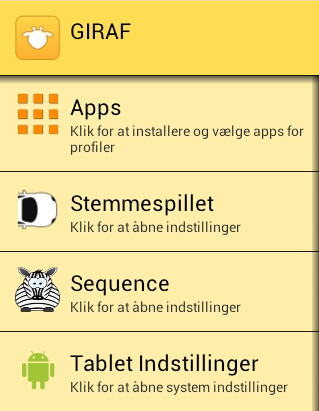
\includegraphics[width=\textwidth]{sprint_one/inconsistent_tab_size_in_settings_panel/example_one}
        \caption{\emph{GIRAF}-tab selected}
        \label{fig:inconsistent_tab_size_in_settings_panel_example_one}
    \end{subfigure}
    \hspace{5em} 
    \begin{subfigure}[t]{0.3\textwidth}
        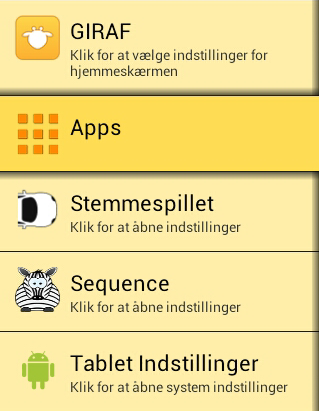
\includegraphics[width=\textwidth]{sprint_one/inconsistent_tab_size_in_settings_panel/example_two}
        \caption{\emph{Apps}-tab selected}
        \label{fig:inconsistent_tab_size_in_settings_panel_example_two}
    \end{subfigure}
    
    \caption{Problem visualized}
    \label{fig:inconsistent_tab_size_in_settings_panel_example}
\end{figure}

A way to solve the problem would be to always show the description, however this does not make much sense because the description is used to indicate what the user might expect to find under the different tabs. For instance the description for the \emph{GIRAF}-tab reads \translated{Klik for at vælge indstillinger for hjemmeskærmen}{Click to choose settings for the home screen}. This text does not make much sense to show when the \emph{GIRAF}-tab is already selected because of two reasons, namely that a click cannot be made since the tab is already active. Besides this, the content corresponding to the settings-tab is shown to the user, so the user could just look at what settings are available and should not need any further instructions to what is available. \\

Another idea would be to remove the descriptions and make the headlines more descriptive. This is a good approach since the only motivation for the existence of the descriptions is the somewhat vague headlines. Let us for instance consider the \emph{GIRAF}-headline. This headline needs a description since it is very unclear what the user might find under this tab. However, if the tab were to be renamed to \translated{Generelt}{General} the user will have a much better understanding of the content of this tab. Besides this, let us consider the tabs \emph{Stemmespillet} and \emph{Sequence}. These two tabs share the same description \translated{Klik for at åbne indstillinger}{Click to open settings}. This description is very basic and vague and thus not needed. Besides this, the user should already be aware that the different tabs will open different setting panes. \\

\figref{fig:inconsistent_tab_size_in_settings_panel_example_solution} shows the implemented solution. It is clear to see that the tab size is consistent and no unclear description texts are shows. Besides this, both the text and the icon has been vertically aligned accordingly to the tab. The first tab has been relabeled to \translated{Generelt}{General}, while the second tab has been relabeled to \translated{Aktive applikationer}{Active applications}.

\begin{figure}[!htbp]
    \centering

    \begin{subfigure}[t]{0.3\textwidth}
        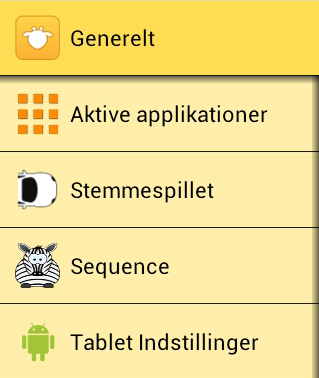
\includegraphics[width=\textwidth]{sprint_one/inconsistent_tab_size_in_settings_panel/example_three}
        \caption{\emph{Generel}-tab selected}
        \label{fig:inconsistent_tab_size_in_settings_panel_example_one_solution}
    \end{subfigure}
    \hspace{5em} 
    \begin{subfigure}[t]{0.3\textwidth}
        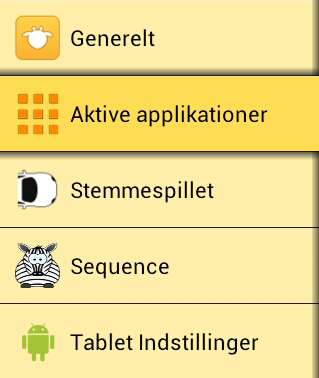
\includegraphics[width=\textwidth]{sprint_one/inconsistent_tab_size_in_settings_panel/example_four}
        \caption{\emph{Aktive applikationer}-tab selected}
        \label{fig:inconsistent_tab_size_in_settings_panel_example_two_solution}
    \end{subfigure}
    
    \caption{Solution visualized}
    \label{fig:inconsistent_tab_size_in_settings_panel_example_solution}
\end{figure}

%!TEX root = ../../../super_main.tex

\section{Reengineering the Application Grid}
\label{sec:reengineering_of_application_grid}
When the \launcher of the \giraf system is being used, and the user presses the drawer on the left-hand side (see \figrefpage{fig:initial_launcher}), the application container becomes smaller as a result of the drawer moving on the screen. The resulting smaller area has to be repopulated with icons, since the icons are no longer within the boundaries of the screen as seen in \figref{fig:overflow_problem}. Furthermore, the application window currently has a fixed size, while the user is able to select as many applications as he/she wants. This means that if too many applications are chosen, they will surpass the size of the window, and therefore be pushed out of the window. The applications are currently being placed in the \launcher by using \androidinline{LinearLayout}s placed in rows, which then individually contain an amount of icons respective to the icon size. This has a serious effect on performance and smoothness of the \launcher. 

\begin{figure}[!htbp]
    \centering
    \begin{subfigure}[t]{0.3\textwidth}
        \centering
        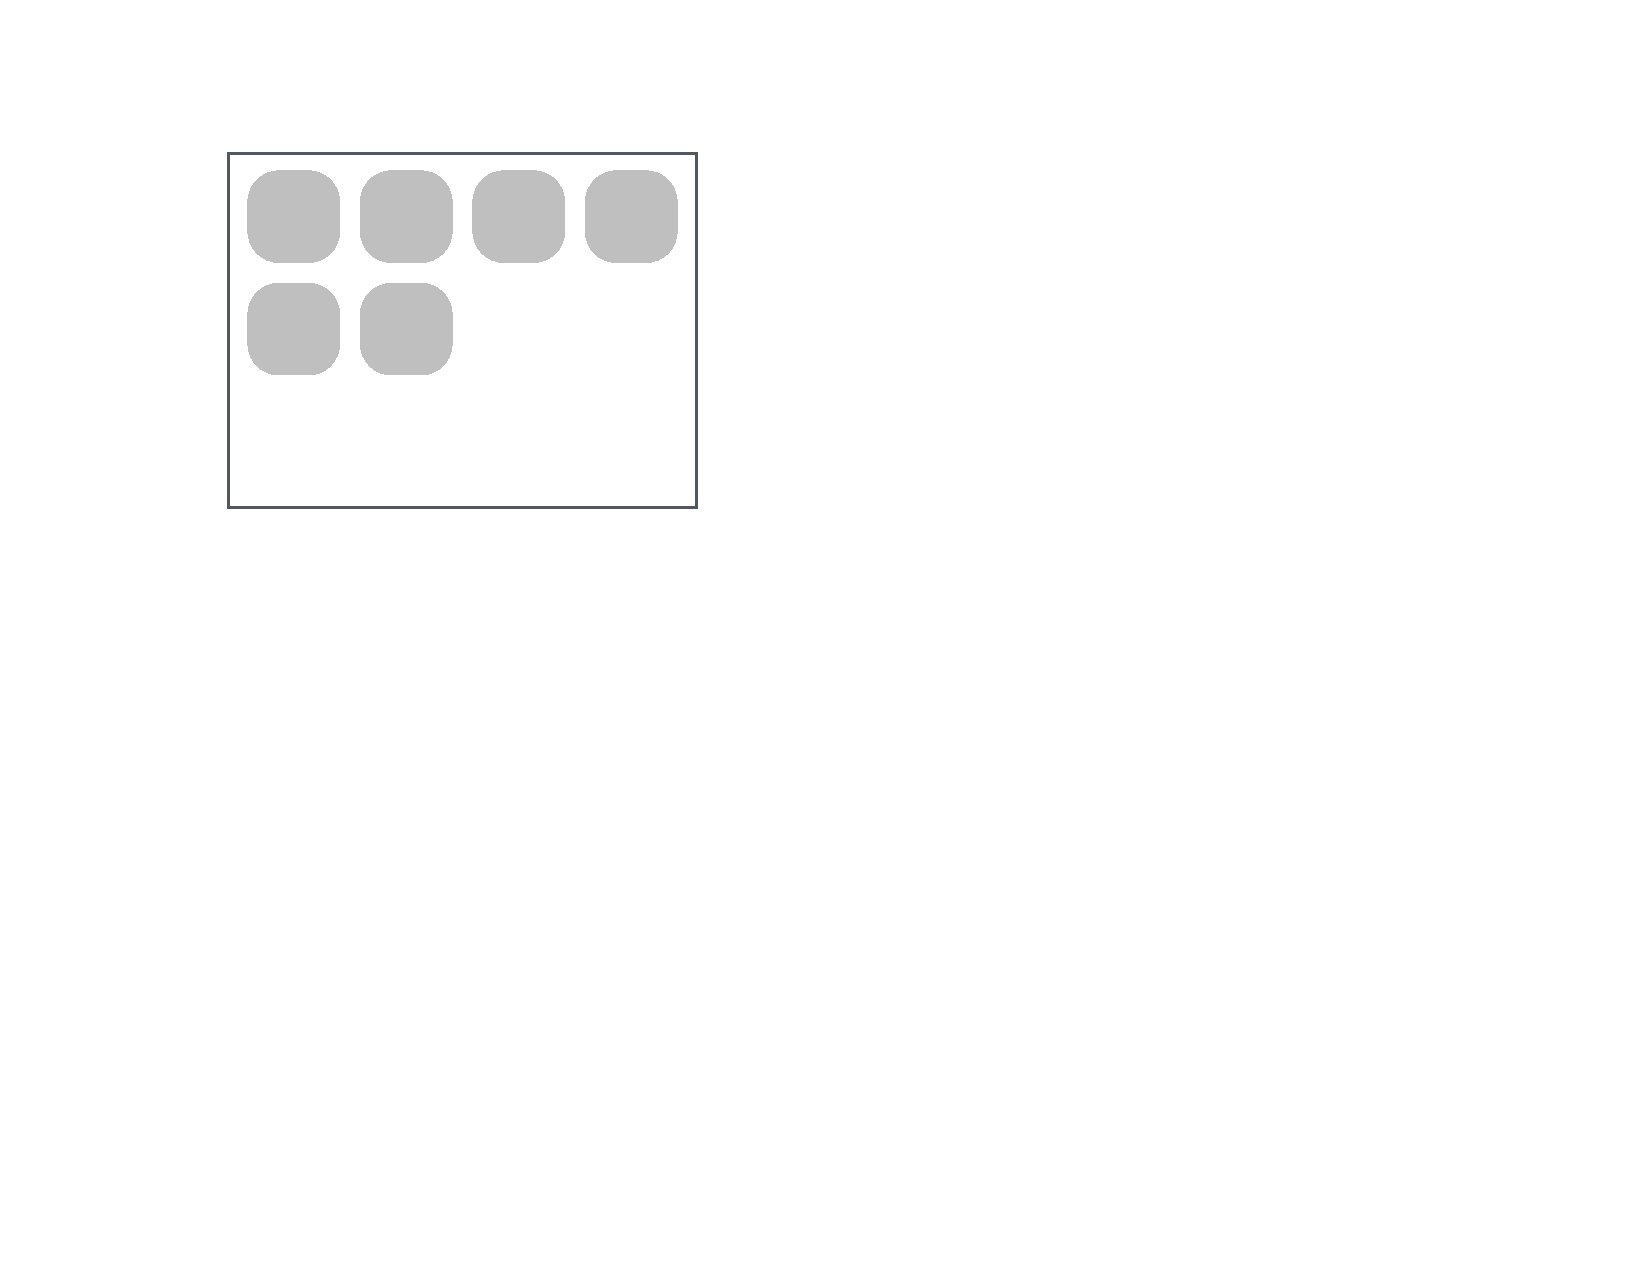
\includegraphics[width=0.7\textwidth]{sprint_one/reengineering_of_application_grid/overflow_problem_small}
        \caption{Small sized application icons}
        \label{fig:overflow_problem_small}
    \end{subfigure}
    \hspace{5em} 
    \begin{subfigure}[t]{0.3\textwidth}
        \centering
        
\includegraphics[width=\textwidth]{sprint_one/reengineering_of_application_grid/overflow_problem_large}
        \caption{Large sized application icons}
        \label{fig:overflow_problem_large}
    \end{subfigure}
    
    \caption{Overflow of application icons}
    \label{fig:overflow_problem}
\end{figure}

The application grid has a setting in the settings menu which allows the user to configure the icon size of the applications shown in the \launcher. The icon size is adjusted by pulling the \androidinline{SeekBar} (slider). This settings menu can be seen in \figref{fig:preference_screen_old}.

\begin{figure}[!htbp]
    \centering
    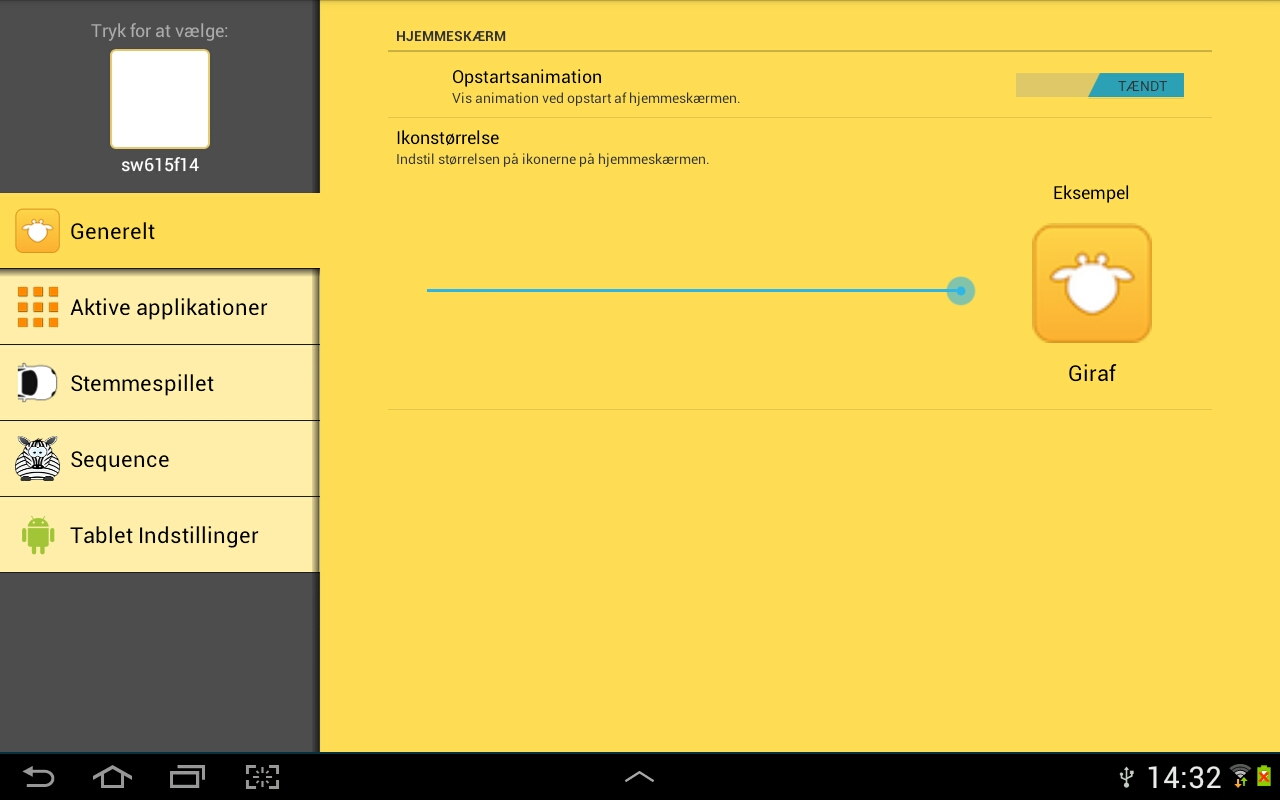
\includegraphics[width=\textwidth]{sprint_one/reengineering_of_application_grid/preference_screen_old}
    \caption{Old preference screen}
    \label{fig:preference_screen_old}
\end{figure}

The \androidinline{LinearLayout} views that are created fit as many icons of the given size inside as possible, while staying within the width of the screen. This is some ``hack'' method that has been implemented in order to allow users to manually change how many icons they want to see in the \launcher. This solution is bad, because instead of changing the actual amount of icons on the screen, the items are just scaled down so more of them can fit on the screen with no indication of how many icons you will now see. \todo{Inddrag kunderne i den her paragraph, fortæl at det en user story for dem}.
\\\\
The creation of \androidinline{LinearLayout} views gives the user a poor experience when interacting with the application, and we would therefore like to improve the \launcher application such that it uses a \androidinline{ViewPager} which contains a grid structure instead. An implementation using \androidinline{GridLayout} is preferable compared to rows of \androidinline{LinearLayout} views, since it is easier to build and populate with icons, which should result in increased performance. A \androidinline{ViewPager} is the standard way of allowing the user to page between screens of applications in other \launcher activities, which is desirable since it gives the user a consistent experience with comparable devices they use. Furthermore, a \androidinline{ViewPagerIndicator} is added to the bottom of the screen, so users have a clear overview of how many pages of applications there are, and how far they have progressed in the paging. The implemented \androidinline{ViewPagerIndicator} comes from an external library\parencite{view_pager_indicator_avianey}, since there is no standard implementation of such a widget in Android. \todo{In this paragraph it is unclear that we actually did this, rewrite such that it is clear.}
\\\\
The functionality in the settings menu that allowed users to change the size of icons has been replaced with the possibility of changing the \launcher grid size. The icon preview in the settings menu now shows an example grid instead. The new setting allows the user to change the size of the grid directly, instead of using the aforementioned indirect icon-resize method. The new settings menu can be seen in \figref{fig:preference_screen_new}.

\todo{Write about the limitation of this settings, we have preset amount of settings. Also mention that we considered two sliders.}

\begin{figure}[!htbp]
    \centering
    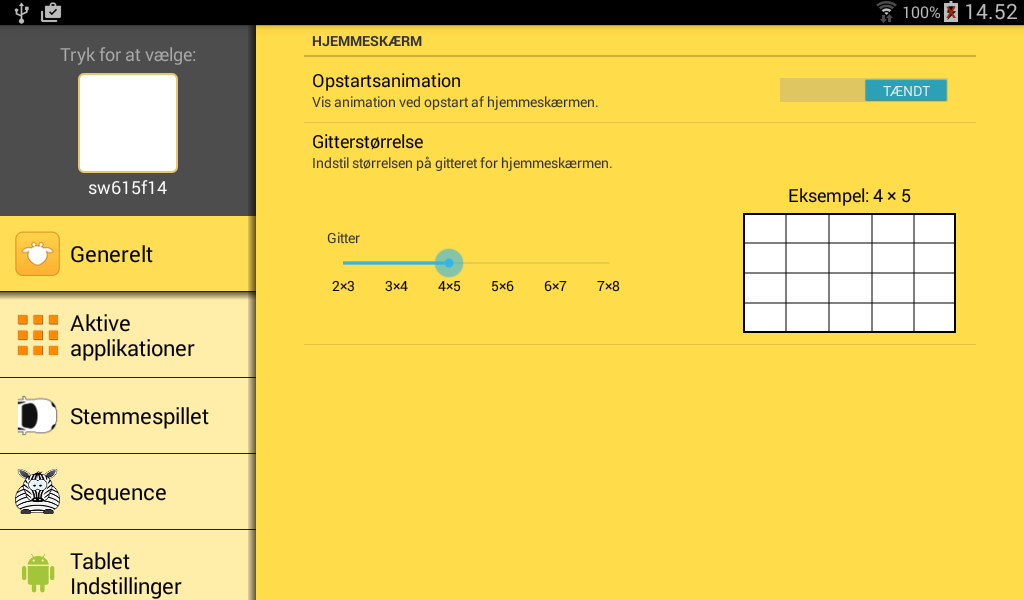
\includegraphics[width=\textwidth]{sprint_one/reengineering_of_application_grid/preference_screen_new}
    \caption{New preference screen}
    \label{fig:preference_screen_new}
\end{figure}

%!TEX root = ../../../super_main.tex
\section{Wrong User Permissions}
\label{sec:wrong_user_permissions}

In the \giraf-applications, there exists three different profile-types, namely \emph{Administrator}, \emph{Guardian}, and \emph{User}. Administrators have the widest permissions, and are allowed to create guardians and users. Guardians can administrate a subset of the users, for instance the users connected to a specific institution, or part of an institution. Users are allowed to use different applications, namely the ones that have been added to their profile by one of their guardians. 
\\\\
However, these different profile-types are not enforced correctly in the \launcher application. Currently, guardian and user profiles have access to the same features. For instance, a regular user may access the settings-panel and choose which applications that should be accessible for that particular user. This feature should only be available for guardian and administrator profiles.
\\\\
Before a guardian hands the tablet to a user, the guardian needs to switch profile to that specific user, so that the system knows what features should be available. Only guardians should be allowed to switch profiles. Currently all profile types are able to switch profiles, meaning that regular users can switch to a guardian profile and thereby gain access to parts of the application that should otherwise be unavailable.
\\\\
We fixed the problem by adding a simple check to profile-type of the current user. The buttons which allowed for switching profiles and settings would then be disabled if the current user is not a guardian or administrator.

%!TEX root = ../../../super_main.tex
\section{Settings Alignment}
\label{sec:settings_alignment}

The settings tab in the \launcher contains the different settings for the user. We noticed during the development, that some of the settings in the panel are not aligned, which gives a bad user impression. We are able to confirm in the code, that the misplacement of the settings is caused by the way a \androidinline{SwitchPreference} is made in Android. By default a \androidinline{SwitchPreference} contains a picture to the left, then some text, and then a switch. As a result, the text is moved to the right to accommodate for the fact that a picture can be present. We intend to change it so that all the settings in the settings panel are aligned to the left side, such that the panel has a consistent and smooth look. The look of the panel with misplaced settings can be seen in \figref{fig:settings_alignment_bad}.

\begin{figure}[!htbp]
    \centering
    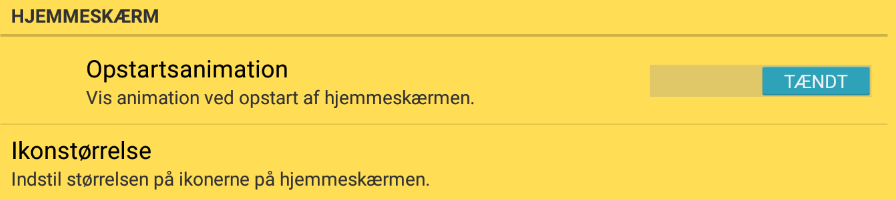
\includegraphics[width=\textwidth]{sprint_one/settings_alignment/bad_alignment}
    \caption{Unaligned settings}
    \label{fig:settings_alignment_bad}
\end{figure}

\subsection{Solution} 
\label{sub:settings_alignment_solution}
We do not want to use pictures as an indicator for our SwitchPreference, so we create our own \androidinline{SwitchPreference} subclass. This allows us to change the visibility of the hidden picture to be ``GONE'' instead. With the picture being gone, the text is able to use the space otherwise reserved for the picture, and nicely align with the settings below it. The panel with properly aligned settings can be seen in \figref{fig:settings_alignment_good}

\begin{figure}[!htbp]
    \centering
    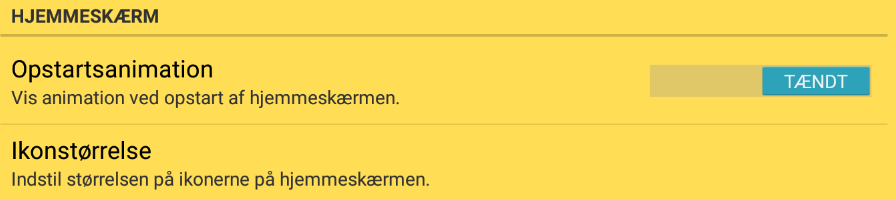
\includegraphics[width=\textwidth]{sprint_one/settings_alignment/good_alignment}
    \caption{Aligned settings}
    \label{fig:settings_alignment_good}
\end{figure}

%!TEX root = ../../../super_main.tex
\section{Button Inconsistency}
\label{sub:button_inconsistency}

The graphical design of the GUI was found to be very inconsistent in general around the \giraf-software suite. This issue was discovered by the \emph{SW606F15} group, who is the group responsible for user requirements and the graphical design guide of the project. \\

In cooperation with this group, it was found that the implementations of the GUI-components that existed needed refactoring based on the code quality and structure of the existing code base of GUI-components. \\

One of the problems found by \emph{SW606F15} is illustrated in \figref{fig:button_inconsistency} where it can be seen that the settings button (top most button) and the logout button (lower most button) are very inconsistent in the graphical design. \\

\begin{figure}[!htbp]
    \centering
    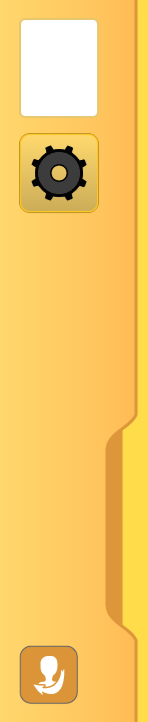
\includegraphics[width=0.1\textwidth]{sprint_one/enforce_design_guide_in_settings/button_inconsistency}
    \caption{Example of inconsistent Buttons}
    \label{fig:button_inconsistency}
\end{figure}

This motivated \emph{SW606F15} to create a graphical design document which will be used to enforce a standard for the GUI, and which can be found in their report\footnote{This report has not yet been published, and we are therefore unable to cite it properly}. Furthermore, this design flaw was found in the GUI of the \launcher, which made us commit to the job of solving this problem. \\

To solve the button inconsistency, a standardized button should be developed. This standard for buttons should correspond to the looks and feel described in the design document created by group \emph{SW606F15}. \\

At first, the design document indicated that there should exist different button types. Each type should have a specific background color associated with it. For instance, buttons with user-actions should have a brown background as seen in \figref{fig:ugly_and_beautiful_buttons_example_one}. However, after implementing this feature, it was discovered that the users at \emph{Birken} did not like these new buttons, and would rather keep the look of the old buttons as seen in \figref{fig:ugly_and_beautiful_buttons_example_two}. However, consistency should still be enforced. This allows for consistent icons and background colors throughout the applications.\\

\begin{figure}[!htbp]
    \centering

    \begin{subfigure}[t]{0.3\textwidth}
    	\centering
        
\includegraphics[width=0.3\textwidth]{sprint_one/ugly_and_beautiful_buttons/button_redesign_beautiful}
        \caption{Colorful buttons}
        \label{fig:ugly_and_beautiful_buttons_example_one}
    \end{subfigure}
    \hspace{5em} 
    \begin{subfigure}[t]{0.3\textwidth}
    	\centering
        
\includegraphics[width=0.3\textwidth]{sprint_one/ugly_and_beautiful_buttons/button_redesign_ugly}
        \caption{Yellow buttons}
        \label{fig:ugly_and_beautiful_buttons_example_two}
    \end{subfigure}
    
    \caption{Solutions visualized}
    \label{fig:ugly_and_beautiful_buttons_example_solution}
\end{figure}

To create the standardized button, a set of graphical icons were made by group \emph{SW606F15}. These icons were then combined with a rounded square with a gradient background with the colors corresponding to the old buttons. All of this was made in the \gc-module, which means that all applications are allowed to use this button. It is however still possible to use wrong icons, but we hope that the other groups will start to use this new button in their projects. \\

Buttons are not the only thing that is inconsistent in the design, however we did not have enough time to create any other standardized components. \\


%!TEX root = ../../../super_main.tex

\section{Unused Drawer}
\label{sec:unused_drawer}

When we took over the \launcher project, the sidebar contained a drawer that could be opened. During the development it was discovered, by contact with the customers, that the drawer was unused and undesired. The fact that the drawer could be opened was indicated by the handle that can be seen in \figref{fig:button_inconsistency}. In order to accommodate for the fact that the drawer is redundant, it was decided to redesign it such that it did not seem clickable. This was achieved by removing the graphical indication of a drawer (see \figref{fig:ugly_and_beautiful_buttons_example_solution}) and removing the \androidinline{onClickListener} on the drawer such that it does not move.  

%!TEX root = ../../../super_main.tex

\section{Missing Apps in Application Grid}
\label{sec:missing_apps_racecondition}

We revealed an issue in the application grid, specifically with the background tasks that loads the applications and their icons. The application grid in the \launcher's Homeactivity would sometimes not show the applications. This issue occurs when the \launcher is to load its applications upon startup. The \launcher starts a background task in its onResume method which loads and prepares the applications to be shown.\\

This bug happens when the onResume method of the Homeactivity checks a boolean variable called \androidinline{mIsAppsContainerInitialized}, which was used in the previous solution to populating the application grid (see \secref{sec:reengineering_of_application_grid}). The previous solution included rebuilding a complicated layout called \androidinline{AppsContainer}, based on \androidinline{LinearLayout} objects, every time the grid had to change. This layout was built on a background thread in a \androidinline{LoadHomeActivityApplicationTask}. Once the layout was completed on the background thread, the variable mIsAppsContainerInitialized was set to true. A check on the variable was then performed to verify whether or not the application screen should be reloaded.

\begin{figure}[!htbp]
    \centering
    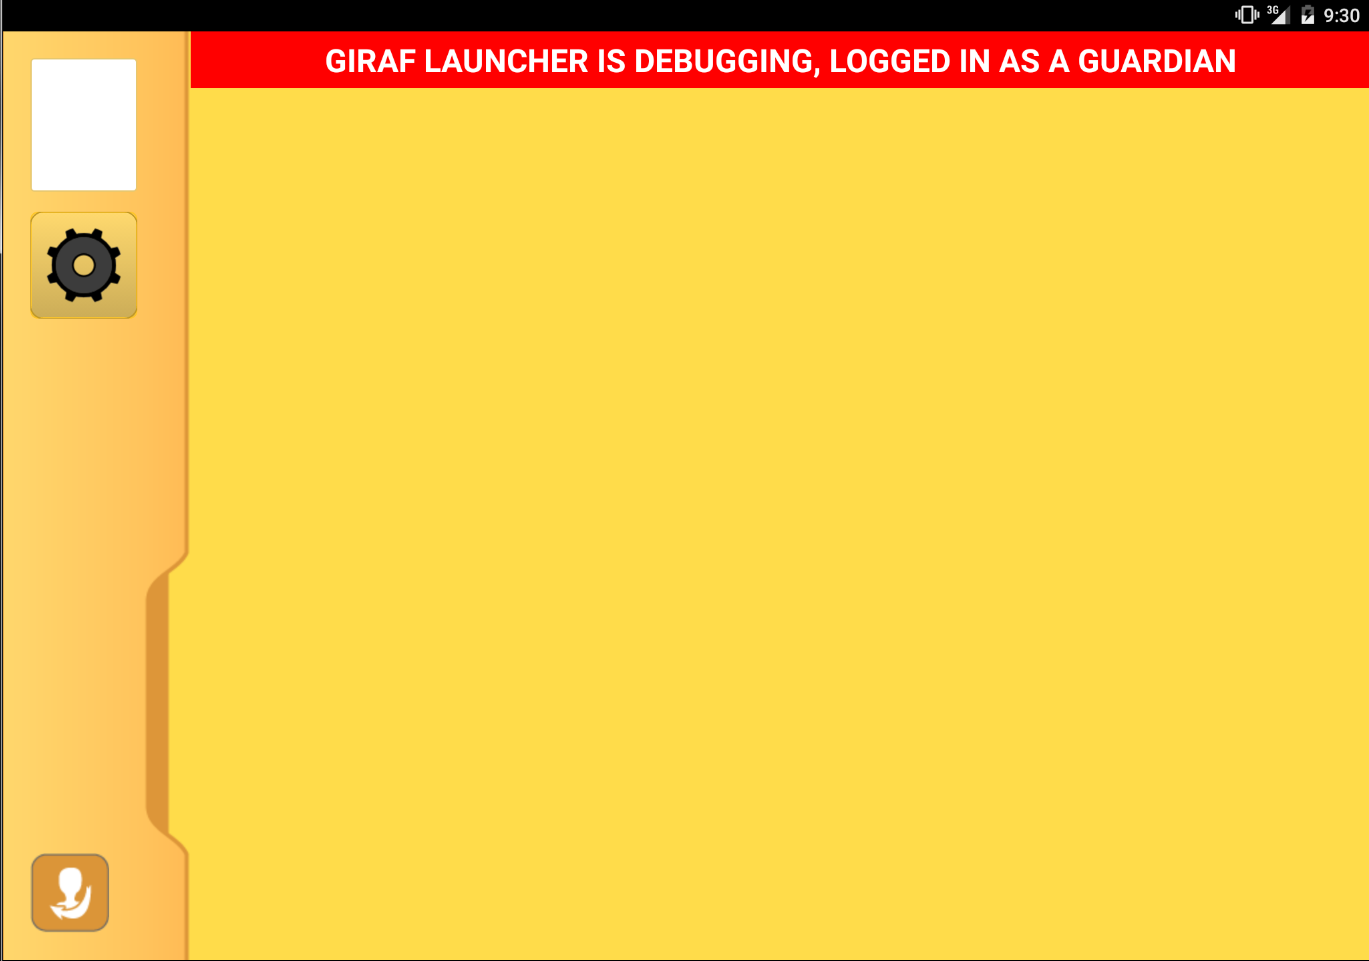
\includegraphics[width=\textwidth]{sprint_one/missing_app_icons/empty_app_icon_screen}
    \caption{Missing Apps}
    \label{fig:missing_apps}
\end{figure}

\subsection{Solution}
\label{sub:missing_apps_racecondition_solution}

The check on \androidinline{mIsAppsContainerInitialized} still happened after we implemented the changes described in \secref{sec:reengineering_of_application_grid}, as it did not seem to have any effect in most cases. Since it has been discovered that errors sometimes happen because of this check, and we no longer have any need to verify that we are done building any layouts, the piece of code has been removed. 

